%
% General structure for the revdetua class:
%
\documentclass[longpaper, english, final, times]{revdetua}
%
% Valid options are:
%
%   longpaper --------- \part and \tableofcontents defined
%   shortpaper -------- \part and \tableofcontents not defined (default)
%
%   english ----------- main language is English (default)
%   portugues --------- main language is Portuguese
%
%   draft ------------- draft version
%   final ------------- final version (default)
%
%   times ------------- use times (postscript) fonts for text
%
%   mirror ------------ prints a mirror image of the paper (with dvips)
%
%   visiblelabels ----- \SL, \SN, \SP, \EL, \EN, etc. defined
%   invisiblelabels --- \SL, \SN, \SP, \EL, \EN, etc. not defined (default)
%
% Note: the final version should use the times fonts
% Note: the really final version should also use the mirror option
%

\usepackage{amsmath, amssymb}
\usepackage{enumitem}
\usepackage{booktabs} % To thicken table lines
%\usepackage{longtable}
\usepackage{arydshln}
\usepackage{graphicx}
\usepackage{dblfloatfix} % fix for table placement
\usepackage{multirow}
\usepackage{subfigure}

%% DIRECTORY TREE REPRESENTATION
\usepackage{forest}

\begin{document}
	
	%\Header{Volume}{Number}{Month}{Year}{InitialPage}
	% Note: the month must be in Portuguese
	
	\title{Probabilistic Counters}
	\author{ABLORDEPPEY Prosper} % or \author{... \and ...}
	\maketitle
	
	\begin{abstract}% Note: in English
		The goal is to count the number of occurrences of letters in text files and, for instance, identify the most common ones. Three types of counters were analyzed. The \textit{Exact Counter}; which provides the exact count or frequency of each letter present in the text, the \textit{Fixed Probability Counter}, with probability $p=\frac{1}{2}$, whose counter value has a 50\% chance of being increased on future occurrences. The last counting method considered, being the \textit{Decreasing Probability Counter} where on future occurrence of a letter, the probability of increasing the counter value decreases. Given the $k'th$ occurrence, this probability  is defined as $\left(\frac{1}{\sqrt{2}^k}\right)$.
	\end{abstract}
	
%	\begin{resumo}% Note: in Portuguese
%		...
%	\end{resumo}
	
%	\begin{keywords}% Note: in English (optional)
%		\begin{enumerate}
%			\item Register :- A table with counter or estimate entries.
%			\item Minimum Space Required :- To store counter value $k$ was computed as $\lceil log2(k)\rceil$.
%			\item For Estimates computation, we developed two (2) derivations;
%			\item Estimates from counter averages :- these are estimates computed from applying the estimation function to the counter averages.
%			\item Average of Counter Estimates :- These estimates are computed from taking the average of estimates for all the experiment.
%		\end{enumerate}
%	\end{keywords}
	
	
	\section*{Project Outline}
		The outline of the project in order is given as.
		\begin{itemize}
			\item Introduction
			\item Project Directory Structure
			\item A Midsummer Nights Dream
			\item Conclusion
		\end{itemize}

	
	\section{Introduction}
		The literary works considered in this project are two (2) works of \textbf{Shakespeare} with each, translated in three (3) different languages \textit{English, French} and \textit{German}.
		The titles of these works in English are;
		\begin{enumerate}
			\item A Midsummer Nights Dream
			\item Hamlet
		\end{enumerate}
	
		
	\section{Project Directory Structure}
		The folder structure for this project is graphically given in Fig. (\ref{figure:projectDirectoryStructure}). 
		From the representation, the project has three (3) directories and the \textit{ProbabilityCounters} python notebook file. Detailed description is presented below;
		\begin{figure}[!ht]
			\begin{center}
				\begin{forest}
					for tree={
						font=\ttfamily,
						grow'=0,
						child anchor=west,
						parent anchor=south,
						anchor=west,
						calign=first,
						edge path={
							\noexpand\path [draw, \forestoption{edge}]
							(!u.south west) +(7.5pt,0) |- node[fill,inner sep=1.25pt] {} (.child anchor)\forestoption{edge label};
						},
						before typesetting nodes={
							if n=1
							{insert before={[,phantom]}}
							{}
						},
						fit=band,
						before computing xy={l=15pt},
					}
					[Project-Two(2)
					[shakespeare
					[hamlet-english.txt]
					[hamlet-french.txt]
					[hamlet-german.txt]
					[...]
					]
					[output
					[hamlet-english\_fixed\_counter.csv]
					[hamlet-english\_fixed\_estimate.csv]
					[hamlet-english\_decrease\_counter.csv]
					[hamlet-english\_decrease\_estimate.csv]
					[hamlet-english\_exact\_counter.csv]
					[hamlet-english\_exact\_estimate.csv]
					[...]
					]
					[combined
					[hamlet-english\_counter\_combined.csv]
					[hamlet-english\_estimate\_combined.csv]
					[hamlet-french\_counter\_combined.csv]
					[hamlet-french\_estimate\_combined.csv]
					[...]
					]
					[ProbabilityCounters.ipynb]
					]
				\end{forest}
			\end{center}
			\caption{Project Directory Structure}
			\label{figure:projectDirectoryStructure}
		\end{figure}
		
		\begin{itemize}
			\setlength\itemsep{1em}
			\item \textbf{shakespeare directory} :- This folder hosts the two (2) literary works of Shakespeare considered in this project. In total, the folder has $2\cdot 3=6$ literary works since each work has translations in English, French and German. For instance, Hamlet has variations, \textit{hamlet-english, hamlet-french} and \textit{hamlet-german}.
			
			\item \textbf{output directory} :- This directory contains the counter and estimate registers in \textit{csv} format, for each of the two (2) count methods (exact, fixed and decreasing prob). Using each count method, multiple experiments were performed for each of the six (6) literary works. Fifty (50) experiments were performed for fixed and decreasing probability counters and only one (1) experiment was performed for the exact counter since the result for multiple experiments will be same. The counter and estimate values were recorded and presented in the \textit{counter} and \textit{estimate} named csv files respectively. Thus, there are $6\cdot 3\cdot 2=36$ csv files in this directory. For instance, the files as shown for the output directory in Fig. \ref{figure:projectDirectoryStructure} is the output registers for hamlet-english literary work only.\\
			
			Each output counter and estimate register have columns presented in TABLE \ref{table:outputCounterRegister} and TABLE \ref{table:outputEstimateRegister} respectively. 
			\begin{table}[!ht]
				\caption{output counter register}
				\begin{center}
					\begin{tabular}{l|l|l}
						letter&minimum&STD\\
						exp 1&maximum&VAR\\
						$\cdots$&average&estimate\\
						exp 50&average\_percent&
					\end{tabular}
				\end{center}
				\label{table:outputCounterRegister}
			\end{table}
			\begin{table}[!ht]
				\caption{output estimate register}
				\begin{center}
					\begin{tabular}{l|l|l}
						letter&minimum&STD\\
						exp 1&maximum&VAR\\
						$\cdots$&average&\\
						exp 50&average\_percent&
					\end{tabular}
				\end{center}
				\label{table:outputEstimateRegister}
			\end{table}
			
			\item \textbf{combined directory}:- This folder holds the combined counters and estimates registers for each literary work. Since there are two (2) outputs for each literary work, there are in all $6\cdot 2=12$ csv registers in csv format.
			
			Each \textit{counter} csv register contains headings as outlined in TABLE \ref{table:combinedCounterRegister}. These tabulations resulted from counter registers in the output directory.\\
			\begin{table}[!ht]
				\caption{combined counter register}
				\hskip-0.6cm
				\begin{tabular}{l|l|l}
					letter&fixed\_minimum&decrease\_minimum\\
					exact&fixed\_maximum&decrease\_maximum\\
					exact\_percent&fixed\_average&decrease\_average\\
					exact\_bits&fixed\_average\_percent&decrease\_average\_percent\\
					&fixed\_bits&decrease\_bits\\
					&fixed\_estimate&decrease\_estimate\\
					&fixed\_STD&decrease\_STD\\
					&fixed\_VAR&decrease\_VAR\\
					&fixed\_meanAbsError&decrease\_meanAbsError\\
					&fixed\_meanRelError&decrease\_meanRelError\\
				\end{tabular}
				\label{table:combinedCounterRegister}
			\end{table}
		
			Similarly, each \textit{estimate} csv register contains headings as outlined in TABLE \ref{table:combinedEstimateRegister}. These tabulations resulted from estimate registers in the output directory.\\
			\begin{table}[!ht]
				\caption{combined estimate register}
				\hskip-0.6cm
				\begin{tabular}{l|l|l}
					letter&fixed\_minimum&decrease\_minimum\\
					exact&fixed\_maximum&decrease\_maximum\\
					exact\_percent&fixed\_average&decrease\_average\\
					exact\_bits&fixed\_average\_percent&decrease\_average\_percent\\
					&fixed\_bits&decrease\_bits\\
					&fixed\_STD&decrease\_STD\\
					&fixed\_VAR&decrease\_VAR\\
					&fixed\_meanAbsError&decrease\_meanAbsError\\
					&fixed\_meanRelError&decrease\_meanRelError\\
				\end{tabular}
				\label{table:combinedEstimateRegister}
			\end{table}
			
			\item \textbf{ProbabilityCounters.ipynb} \\
				This is the python notebook file generating the \textit{output} and \textit{combined} registers as detailed above. This file implements three (3) classes. Namely
				\begin{itemize}
					\setlength\itemsep{0em}
					\item BaseCounter (IO File Operations)
					\item ApproximateCounters (Counters Implementation)
					\item Combiner (Combined File Generations)
				\end{itemize}
		\end{itemize}
	
	\section{A Midsummer Nights Dream}
		\subsection{English}
			\subsubsection{counters}
				Fig. \ref{fig:aMidsummerNightsDreamEnglishCounter} shows distribution of the counter values for the exact, fixed and decreasing probability counters. It can be observed that the fixed probability counter values are approximately half of the exact counter values. This is due to the fact that the fix probability of increasing counter value on new occurrence is $p=\frac{1}{2}$.  For larger occurrences, the decreasing probability counter slowly updates the counter value as observed in Fig. \ref{fig:aMidsummerNightsDreamEnglishCounterAverage}. This explains why such counter values are insignificant as compared to the fixed probability counter values.\\
				
				Again, the space complexity for the decreasing probability counter is the smallest, followed by the fixed probability counter. The minimum amount of memory (bits) required to store each counter value is also presented in Fig. \ref{fig:aMidsummerNightsDreamEnglishCounterbits}. Though the minimum memory required to store the exact and fixed probability counter values are approximately equal but relatively higher for the exact counter, the decreasing probability counter has slowly increasing memory size, as shown.
				\begin{figure}[h]
					\caption{A Midsummer Nights Dream - English Counters}
					\begin{center}
						\subfigure[Counter Average]{
							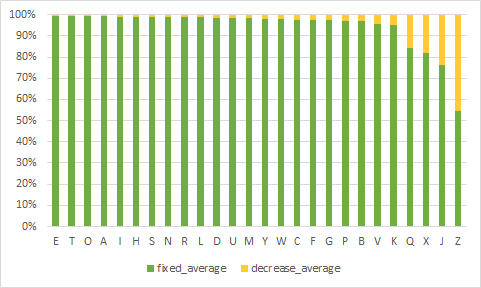
\includegraphics[width=.225\textwidth]{./imgs/aMidsummerNightsDreamEnglishCounterAverage.png}
							\label{fig:aMidsummerNightsDreamEnglishCounterAverage}
						}
						\subfigure[counter minimum space (bits)]{
							\includegraphics[width=.225\textwidth]{./imgs/aMidsummerNightsDreamEnglishCounterbits.png}
							\label{fig:aMidsummerNightsDreamEnglishCounterbits}
						}
					\end{center}
					\label{fig:aMidsummerNightsDreamEnglishCounter}
				\end{figure}
			
			\subsubsection{estimates}
				Fig. \ref{fig:aMidsummerNightsDreamEnglishEstimate} presents the distribution of the estimates. As shown in Fig. \ref{fig:aMidsummerNightsDreamEnglishEstimateAverage}, and Fig. \ref{fig:aMidsummerNightsDreamEnglishCounterEstimate}, estimates computed from taking the average of the counter estimates for all experiments (thus, \ref{fig:aMidsummerNightsDreamEnglishEstimateAverage}) tends to be more closer to the exact number of occurrence for the decreasing probability counter. Both approaches provide similar result for the fixed probability counter. The order of the counters is preserved in both cases.\\
			
				Fig. \ref{fig:aMidsummerNightsDreamEnglishEstimate} shows the average percentage of occurrence for each letter for the various count methods. Using the exact values, the top four (4) most occurring letters are \textit{E-12.5\%, T-8.7\%, O-8.1\%} and \textit{A-7.5\%}. This ranking is preserved for the fixed and decreasing probability counters. Although the decreasing probability estimates recorded slightly higher occurrence percentages, the distribution of these estimates is similar to that of the exact and fixed probability counters. These percentages are consistent with the known standards.\\
				
				Just as with the mean absolute errors, we observe larger mean relative errors for the decrease probability counter as compared to the fixed probability counter. This is so because, the decreasing probability counter used very less memory for counting as opposed to the fixed probability counter, thereby, recording larger errors. \\
				
				We also observe very high variation in estimates for the decreasing probability counter as opposed to the fixed probability counter, as shown in Fig. \ref{fig:aMidsummerNightsDreamEnglishEstimate}.
				\begin{figure}
					\caption{A Midsummer Nights Dream Estimates - English Estimates}
					\begin{center}
						\subfigure[Average of Counter Estimates]{
							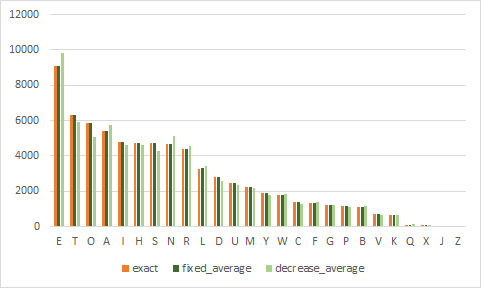
\includegraphics[width=.225\textwidth]{./imgs/aMidsummerNightsDreamEnglishEstimateAverage.png}
							\label{fig:aMidsummerNightsDreamEnglishEstimateAverage}
						}
						\subfigure[Estimates of Counter Averages]{
							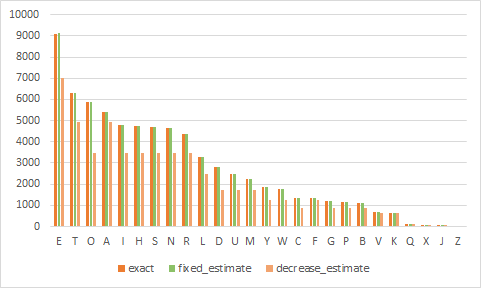
\includegraphics[width=.225\textwidth]{./imgs/aMidsummerNightsDreamEnglishCounterEstimate.png}
							\label{fig:aMidsummerNightsDreamEnglishCounterEstimate}
						}
						\subfigure[Average Occurrence Percentage]{
							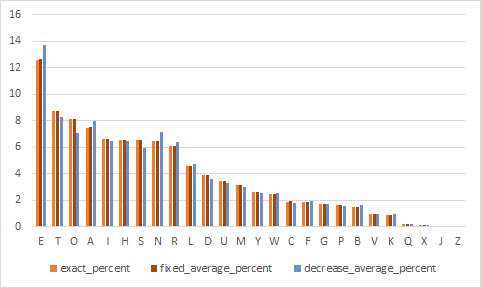
\includegraphics[width=.225\textwidth]{./imgs/aMidsummerNightsDreamEnglishEstimatePercent.png}
							\label{fig:aMidsummerNightsDreamEnglishEstimatePercent}
						}
						\subfigure[Mean Absolute Error]{
							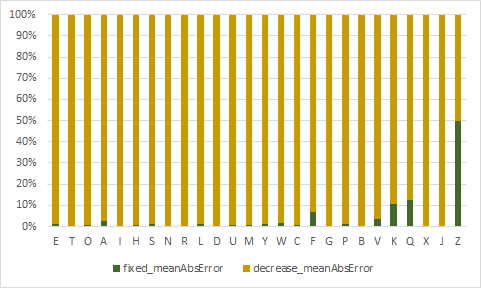
\includegraphics[width=.225\textwidth]{./imgs/aMidsummerNightsDreamEnglishEstimateMeanAbsError.png}
							\label{fig:aMidsummerNightsDreamEnglishEstimateMeanAbsError}
						}
						\subfigure[Mean Relative Error]{
							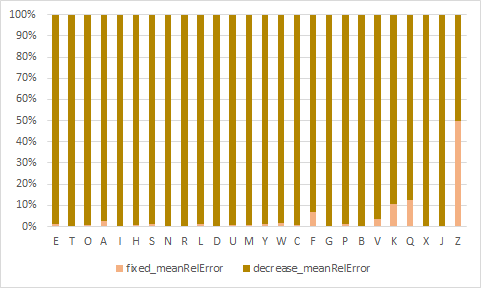
\includegraphics[width=.225\textwidth]{./imgs/aMidsummerNightsDreamEnglishEstimateMeanRelError.png}
							\label{fig:aMidsummerNightsDreamEnglishEstimateMeanRelError}
						}
						\subfigure[Variance]{
							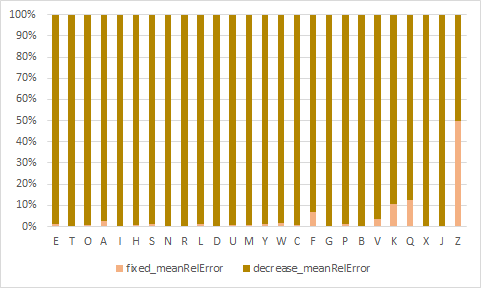
\includegraphics[width=.225\textwidth]{./imgs/aMidsummerNightsDreamEnglishEstimateVAR.png}
							\label{fig:aMidsummerNightsDreamEnglishEstimateVAR}
						}
					\end{center}
					\label{fig:aMidsummerNightsDreamEnglishEstimate}
				\end{figure}
			
			
		\subsection{French}
			Fig. \ref{fig:aMidsummerNightsDreamFrenchCounter} presents the distribution of the counter values, and Fig. \ref{fig:aMidsummerNightsDreamFrenchCounter} shows the corresponding estimates distribution. 
			
			As shown in Fig.  \ref{fig:aMidsummerNightsDreamFrenchCounter}, estimates computed from taking the average of the counter estimates for all experiments also happens to be better estimates than the estimates computed from the average counter values. Both approaches provide similar result for the fixed probability counter. 
			Although there are a few disagreement with the ranking of the most occurring letters for the decrease probability counter estimates, on average, the order is preserved.\\
			
			Fig. \ref{fig:aMidsummerNightsDreamFrenchEstimate} shows the average percentage occurrence for each letter for the various count methods. Using the exact values, the top four (4) most occurring letters are \textit{E-15\%, S-7.8\%, T-7.2\%, N-7.1\%} and \textit{R-7\%}. The least occurrence being $X, Z, W, K$. These rankings are preserved for the fixed and decreasing probability counters for all letters. Although the decreasing probability estimates recorded slightly higher occurrence percentages, the distribution of these estimates is similar to that of the exact and fixed probability counters. These rankings are consistent with known standards.\\
			
			Just as the mean absolute errors, Fig.  \ref{fig:aMidsummerNightsDreamFrenchEstimate} shows larger mean relative errors for the decrease probability counter estimates as compared to the fixed probability counters. This is so because, the decreasing probability counter used very less memory for counting as opposed to the fixed probability counter, thereby, recording larger errors. \\
			
			We also observe very high variation in estimates from the decreasing probability counter as opposed to the fixed probability counter as shown in Fig. \ref{fig:aMidsummerNightsDreamFrenchEstimate}.
		
			\begin{figure}[!h]
				\caption{A Midsummer Nights Dream Counters - French Counter}
				\begin{center}
					\subfigure[counter average]{
						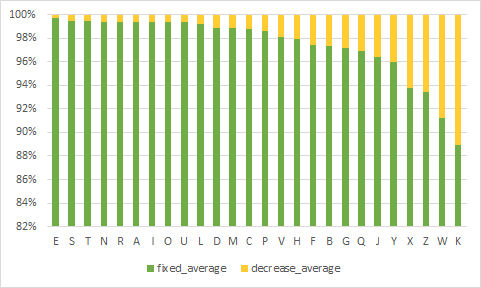
\includegraphics[width=.225\textwidth]{./imgs/aMidsummerNightsDreamFrenchCounterAverage.png}
					}
					\subfigure[counter minimum space (bits)]{
						\includegraphics[width=.225\textwidth]{./imgs/aMidsummerNightsDreamFrenchCounterbits.png}
					}
				\end{center}
				\label{fig:aMidsummerNightsDreamFrenchCounter}
			\end{figure}
		
			\begin{figure}[!h]
				\caption{A Midsummer Nights Dream - French Estimates}
				\begin{center}
					\subfigure[Average of Counter Estimates]{
						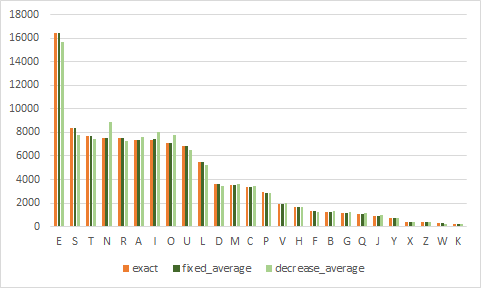
\includegraphics[width=.225\textwidth]{./imgs/aMidsummerNightsDreamFrenchEstimateAverage.png}
					}
					\subfigure[Estimates of Counter Averages]{
						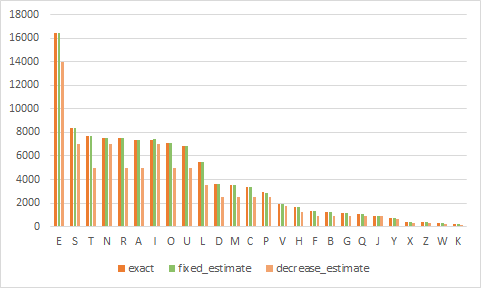
\includegraphics[width=.225\textwidth]{./imgs/aMidsummerNightsDreamFrenchCounterEstimate.png}
					}
					\subfigure[Average Occurrence Percentage]{
						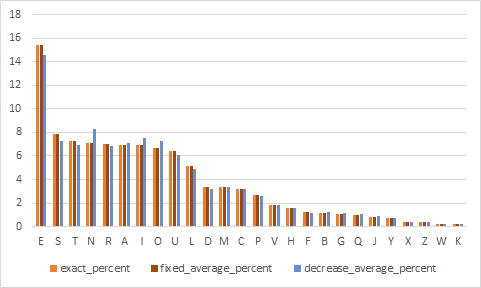
\includegraphics[width=.225\textwidth]{./imgs/aMidsummerNightsDreamFrenchEstimatePercent.png}
					}
					\subfigure[Mean Absolute Error]{
						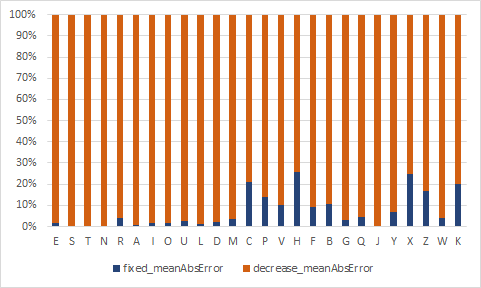
\includegraphics[width=.225\textwidth]{./imgs/aMidsummerNightsDreamFrenchEstimateMeanAbsError.png}
					}
					\subfigure[Mean Relative Error]{
						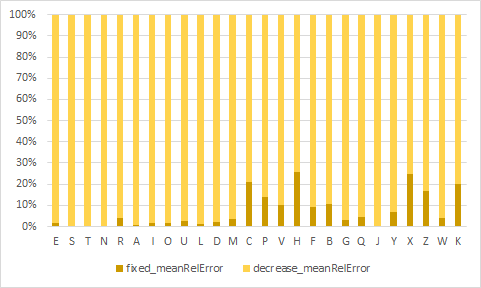
\includegraphics[width=.225\textwidth]{./imgs/aMidsummerNightsDreamFrenchEstimateMeanRelError.png}
					}
					\subfigure[Variance]{
						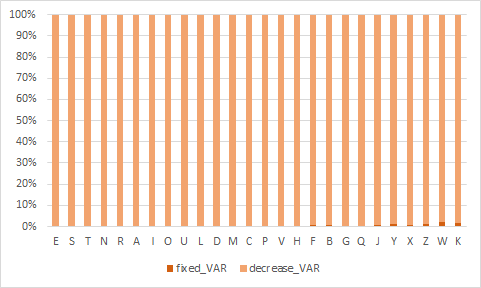
\includegraphics[width=.225\textwidth]{./imgs/aMidsummerNightsDreamFrenchEstimateVAR.png}
					}
				\end{center}
				\label{fig:aMidsummerNightsDreamFrenchEstimate}
			\end{figure}
			
		\subsection{German}
			Fig. \ref{fig:aMidsummerNightsDreamGermanCounter} shows the distribution of the counter values, and Fig. \ref{fig:aMidsummerNightsDreamGermanEstimate} shows the corresponding estimates distribution. 
			
			As shown in Fig.  \ref{fig:aMidsummerNightsDreamGermanCounter}, estimates computed from taking the average of the counter estimates for all experiments also happens to be better estimates than the estimates computed from the average counter values. Both approaches provide similar result for the fixed probability counter. 
			Although there are a few disagreement with the ranking of the most occurring letters for the decrease probability counter estimates, on average, the order is preserved.\\
			
			Fig. \ref{fig:aMidsummerNightsDreamGermanEstimate} shows the average percentage occurrence for each letter for the various count methods. Using the exact values, the top four (4) most occurring letters are \textit{E-15.6\%, N-9.7\%, I-8.7\%, R-6.8\%} and \textit{H-6.3\%}. The least occurrence being $Y, J, Q, X$. These rankings are preserved for the fixed and decreasing probability counters for all letters. Although the decreasing probability estimates recorded slightly higher occurrence percentages, the distribution of these estimates is similar to that of the exact and fixed probability counters. These rankings are consistent with known standards.\\
			
			Just as the mean absolute errors in Fig.  \ref{fig:aMidsummerNightsDreamGermanEstimate} shows larger mean relative errors for the decrease probability counter as compared to the fixed probability counters. This is so because, the decreasing probability counter used very less memory for counting as opposed to the fixed probability counter, thereby, recording larger errors. \\
			
			We also observe very high variation in estimates from the decreasing probability counter as opposed to the fixed probability counter as shown in Fig. \ref{fig:aMidsummerNightsDreamGermanEstimate}.
			
			\begin{figure}[!h]
				\caption{A Midsummer Nights Dream Counters - German Counter}
				\begin{center}
					\subfigure[counter average]{
						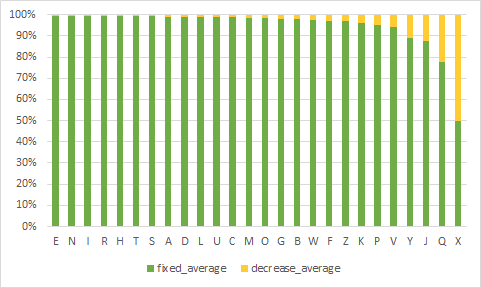
\includegraphics[width=.225\textwidth]{./imgs/aMidsummerNightsDreamGermanCounterAverage.png}
					}
					\subfigure[counter minimum space (bits)]{
						\includegraphics[width=.225\textwidth]{./imgs/aMidsummerNightsDreamGermanCounterbits.png}
					}
				\end{center}
				\label{fig:aMidsummerNightsDreamGermanCounter}
			\end{figure}
		
			\begin{figure}[!h]
				\caption{A Midsummer Nights Dream - German Estimates}
				\begin{center}
					\subfigure[Average of Counter Estimates]{
						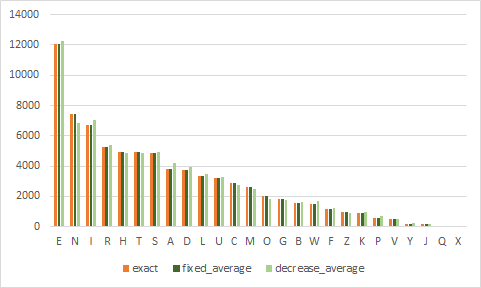
\includegraphics[width=.225\textwidth]{./imgs/aMidsummerNightsDreamGermanEstimateAverage.png}
					}
					\subfigure[Estimates of Counter Averages]{
						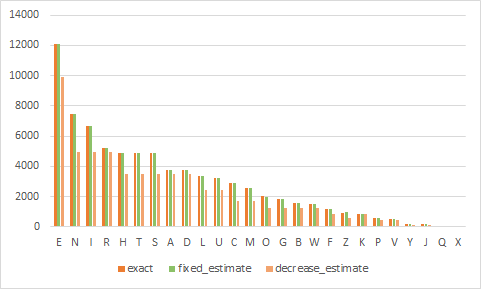
\includegraphics[width=.225\textwidth]{./imgs/aMidsummerNightsDreamGermanCounterEstimate.png}
					}
					\subfigure[Average Occurrence Percentage]{
						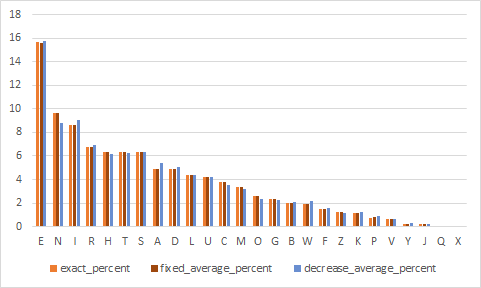
\includegraphics[width=.225\textwidth]{./imgs/aMidsummerNightsDreamGermanEstimatePercent.png}
					}
					\subfigure[Mean Absolute Error]{
						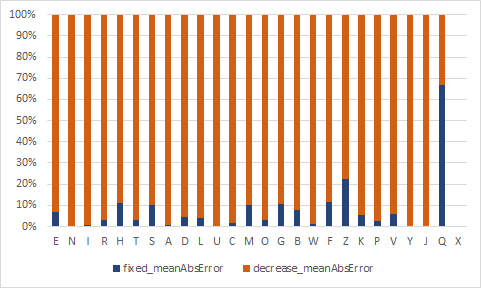
\includegraphics[width=.225\textwidth]{./imgs/aMidsummerNightsDreamGermanEstimateMeanAbsError.png}
					}
					\subfigure[Mean Relative Error]{
						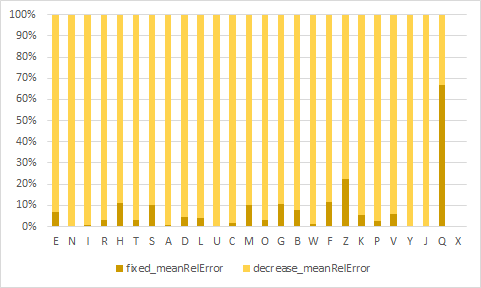
\includegraphics[width=.225\textwidth]{./imgs/aMidsummerNightsDreamGermanEstimateMeanRelError.png}
					}
					\subfigure[Variance]{
						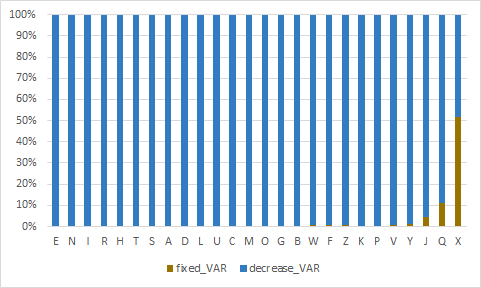
\includegraphics[width=.225\textwidth]{./imgs/aMidsummerNightsDreamGermanEstimateVAR.png}
					}
				\end{center}
				\label{fig:aMidsummerNightsDreamGermanEstimate}
			\end{figure}
			
			
	\section{Hamlet}
		\subsection{English}
			Fig. \ref{fig:hamletEnglishCounter} shows the distribution of counter values for each letter, and Fig. \ref{fig:hamletEnglishEstimate} also shows the distribution of the estimates for each count method. \textit{E,A,O,S,R} happens to be the top five (5) most occurring letters, with percentages \textit{13.6\%, 11.1\%, 9.3\%, 7.8} and  \textit{6.9\%} respectively.\\
			
			There is not significant variation between the estimates from the fixed and decreasing probability estimates. Letters $K$ and $W$ are have similar variations for both counters. \\
			
			The estimates computed from taking the average of estimates for all experiments seem to be a better estimate than those computed via the counter averages, although on average, they record slightly higher values compared to the exact counters values.\\
			
			The relative errors observed for the fixed probability counter are generally low compared to those from the exact counter, but we see an abnormally high error recorded for letter $V$ for the fixed probability counter.\\
			
			From the above, we confirm from the graph the high variation in the estimates for the decreasing probability counter. For letters $K$ and $W$ which occurs the least, we notice similar variation of the computed estimates. \\
			
			Again, the memory size in bits required to store the counters for the decreasing probability counter is very small and increases slowly for larger occurrences.
			\begin{figure}[h]
				\caption{Hamlet Counters - English Counter}
				\begin{center}
					\subfigure[counter average]{
						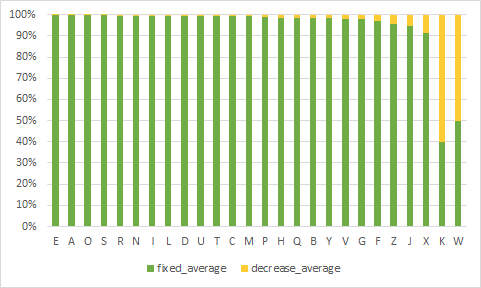
\includegraphics[width=.225\textwidth]{./imgs/hamletEnglishCounterAverage.png}
						\label{fig:hamletEnglishCounterAverage}
					}
					\subfigure[counter minimum space (bits)]{
						\includegraphics[width=.225\textwidth]{./imgs/hamletEnglishCounterbits.png}
						\label{fig:hamletEnglishCounterbits}
					}
				\end{center}
				\label{fig:hamletEnglishCounter}
			\end{figure}
			
			\begin{figure}
				\caption{Hamlet - English Estimates}
				\begin{center}
					\subfigure[Average of Counter Estimates]{
						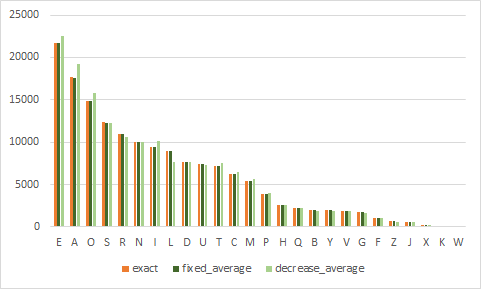
\includegraphics[width=.225\textwidth]{./imgs/hamletEnglishEstimateAverage.png}
					}
					\subfigure[Estimates of Counter Averages]{
						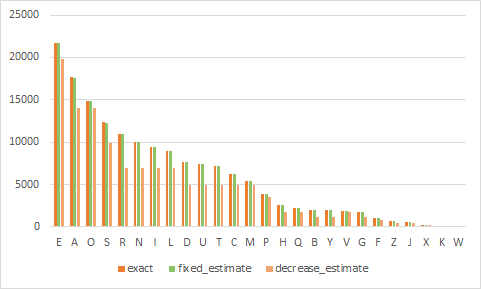
\includegraphics[width=.225\textwidth]{./imgs/hamletEnglishCounterEstimate.png}
					}
					\subfigure[Average Occurrence Percentage]{
						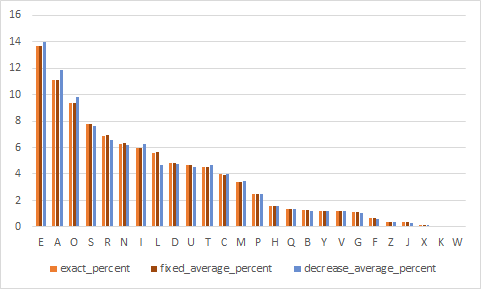
\includegraphics[width=.225\textwidth]{./imgs/hamletEnglishEstimatePercent.png}
					}
					\subfigure[Mean Absolute Error]{
						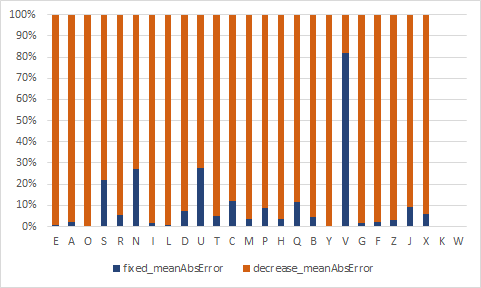
\includegraphics[width=.225\textwidth]{./imgs/hamletEnglishEstimateMeanAbsError.png}
					}
					\subfigure[Mean Relative Error]{
						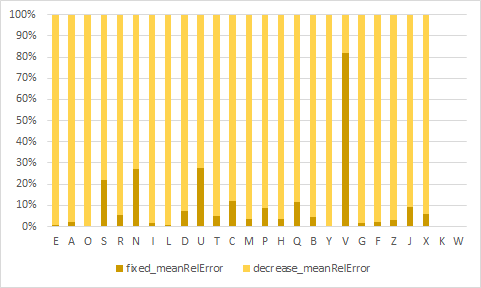
\includegraphics[width=.225\textwidth]{./imgs/hamletEnglishEstimateMeanRelError.png}
					}
					\subfigure[Variance]{
						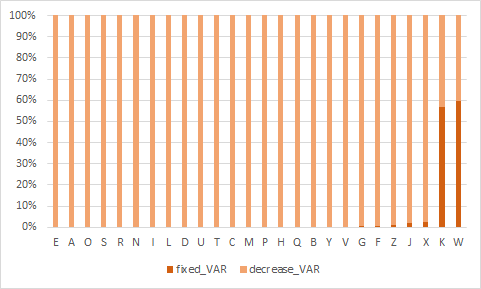
\includegraphics[width=.225\textwidth]{./imgs/hamletEnglishEstimateVAR.png}
					}
				\end{center}
				\label{fig:hamletEnglishEstimate}
			\end{figure}

		\subsection{French}
			Fig. \ref{fig:hamletFrenchCounter} shows the distribution of counter values for each letter. The top five (5) most occurring letters are \textit{E,S,A,N,T}, happens to occur with percentages \textit{16\%, 8.3\%, 7.4\%, 7.3\%} and  \textit{7.2\%} respectively. The least five occurring letters are \textit{X, Z, Y, K, W} .The estimates closer to the exact counter values are those computed from the average of the counter estimates as observed in Fig. \ref{fig:hamletFrenchEstimate}(a). Most variation in the fixed probability counter estimates was recorded for estimate for letter $F$.
			
			Variation in the decrease probability counter estimates is very high for all records.

			\begin{figure}[!h]
				\caption{Hamlet Counters - French Counter}
				\begin{center}
					\subfigure[counter average]{
						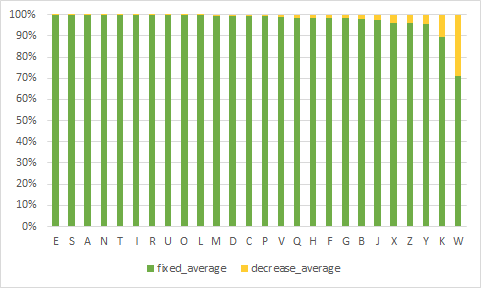
\includegraphics[width=.225\textwidth]{./imgs/hamletFrenchCounterAverage.png}
					}
					\subfigure[counter minimum space (bits)]{
						\includegraphics[width=.225\textwidth]{./imgs/hamletFrenchCounterbits.png}
					}
				\end{center}
				\label{fig:hamletFrenchCounter}
			\end{figure}
	
			\begin{figure}[!h]
				\caption{Hamlet - French Estimates}
				\begin{center}
					\subfigure[Average of Counter Estimates]{
						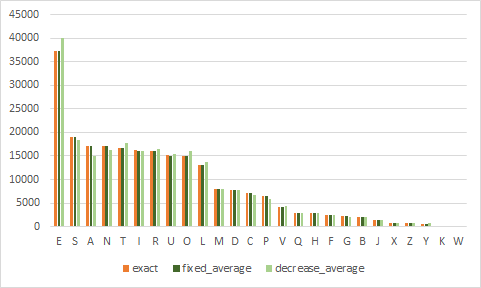
\includegraphics[width=.225\textwidth]{./imgs/hamletFrenchEstimateAverage.png}
					}
					\subfigure[Estimates of Counter Averages]{
						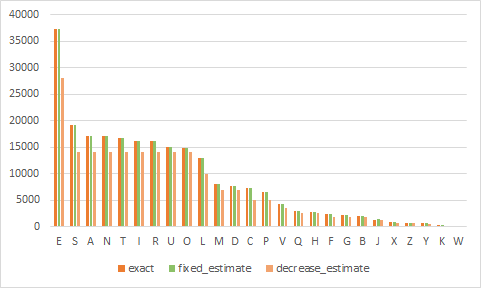
\includegraphics[width=.225\textwidth]{./imgs/hamletFrenchCounterEstimate.png}
					}
					\subfigure[Average Occurrence Percentage]{
						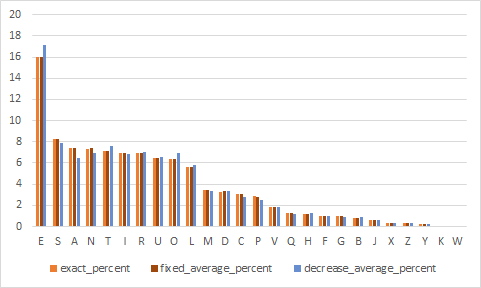
\includegraphics[width=.225\textwidth]{./imgs/hamletFrenchEstimatePercent.png}
					}
					\subfigure[Mean Absolute Error]{
						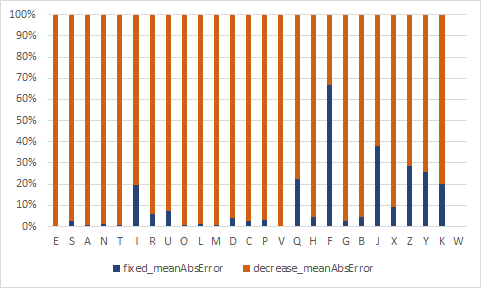
\includegraphics[width=.225\textwidth]{./imgs/hamletFrenchEstimateMeanAbsError.png}
					}
					\subfigure[Mean Relative Error]{
						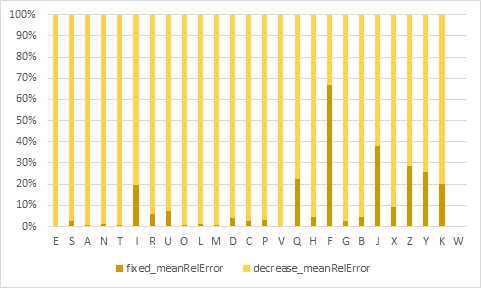
\includegraphics[width=.225\textwidth]{./imgs/hamletFrenchEstimateMeanRelError.png}
					}
					\subfigure[Variance]{
						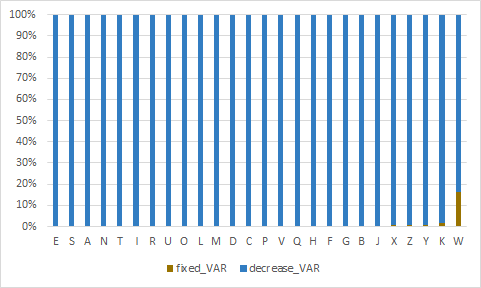
\includegraphics[width=.225\textwidth]{./imgs/hamletFrenchEstimateVAR.png}
					}
				\end{center}
				\label{fig:hamletFrenchEstimate}
			\end{figure}


		\subsection{German}
			Fig. \ref{fig:hamletGermanCounter} shows the distribution of counter values for each letter. The top five (5) most occurring letters are \textit{E,S,A,N,T}, happens to occur with percentages \textit{16\%, 8.3\%, 7.4\%, 7.3\%} and  \textit{7.2\%} respectively. The least five occurring letters are \textit{W, K, X, J, Z} .The estimates closer to the exact counter values are those computed from the average of the counter estimates as observed in Fig. \ref{fig:hamletGermanEstimate}. Most variation in the fixed probability counter estimates was recorded for the letter $W$. \\
			
			The counter averages for the decreasing probability counter increases slowly for higher occurrences, as shown in Fig. \ref{fig:hamletGermanCounter}. The minimum memory (bits) is also constant for large occurrences.
			
			\begin{figure}[!h]
				\caption{Hamlet Counters - German Counter}
				\begin{center}
					\subfigure[counter average]{
						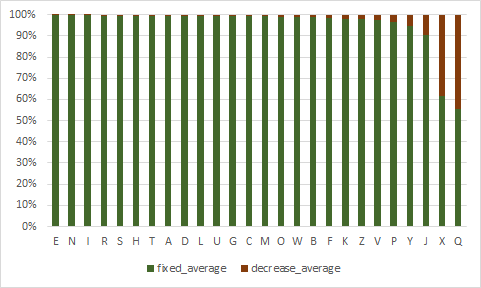
\includegraphics[width=.225\textwidth]{./imgs/hamletGermanCounterAverage.png}
					}
					\subfigure[counter minimum space (bits)]{
						\includegraphics[width=.225\textwidth]{./imgs/hamletGermanCounterbits.png}
					}
				\end{center}
				\label{fig:hamletGermanCounter}
			\end{figure}
		
			\begin{figure}[!h]
				\caption{Hamlet - German Estimates}
				\begin{center}
					\subfigure[Average of Counter Estimates]{
						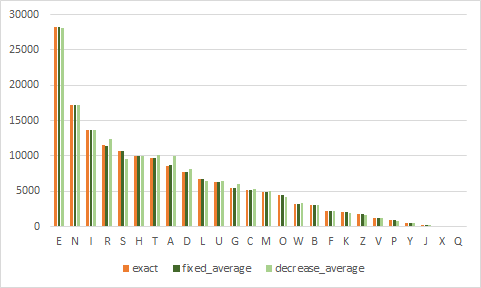
\includegraphics[width=.225\textwidth]{./imgs/hamletGermanEstimateAverage.png}
					}
					\subfigure[Estimates of Counter Averages]{
						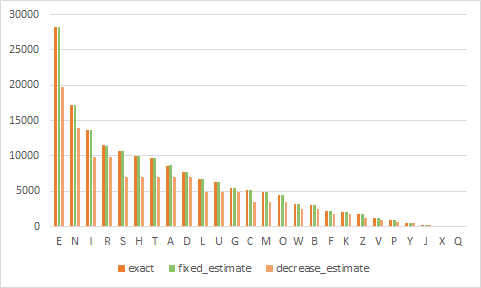
\includegraphics[width=.225\textwidth]{./imgs/hamletGermanCounterEstimate.png}
					}
					\subfigure[Average Occurrence Percentage]{
						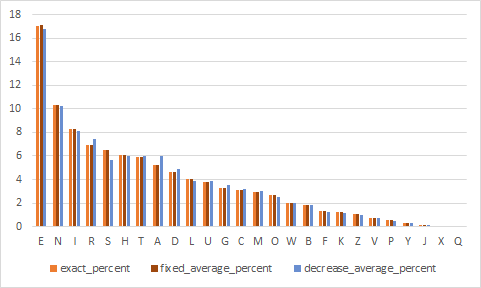
\includegraphics[width=.225\textwidth]{./imgs/hamletGermanEstimatePercent.png}
					}
					\subfigure[Mean Absolute Error]{
						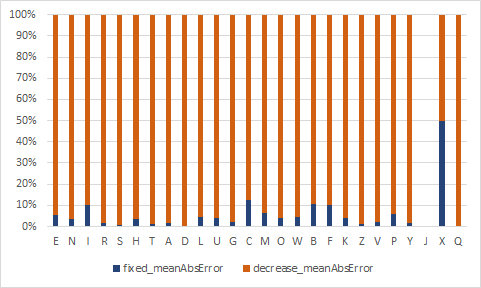
\includegraphics[width=.225\textwidth]{./imgs/hamletGermanEstimateMeanAbsError.png}
					}
					\subfigure[Mean Relative Error]{
						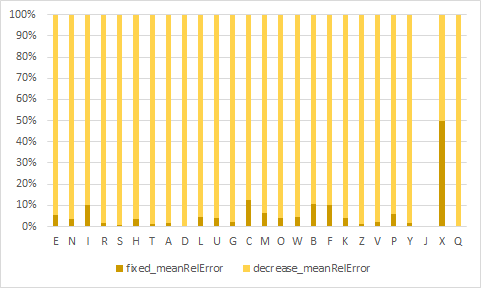
\includegraphics[width=.225\textwidth]{./imgs/hamletGermanEstimateMeanRelError.png}
					}
					\subfigure[Variance]{
						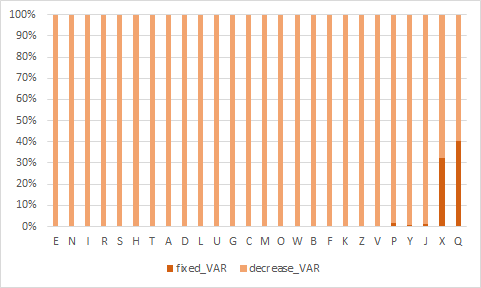
\includegraphics[width=.225\textwidth]{./imgs/hamletGermanEstimateVAR.png}
					}
				\end{center}
				\label{fig:hamletGermanEstimate}
			\end{figure}
		

	\section{Conclusion}
		From the above results and analysis, we arrive at the following conclusion;
		\begin{itemize}
			\setlength\itemsep{1em}
			\item Estimates computed by taking the average of all estimates yields better result as compared to those obtained from average of the counter values.
			\item The top (10) most frequent English letters in a standard text documents are \textit{\{E,T,A,O,I,N,S,R,H,L\}}, confirmed by our results in this presentation \cite{letter_frequency}.
			\item Also, the first ten (10) most frequent French letters as observed in the analysis are \textit{\{E,S,A,N,T,I,R,O,U,L\}}. These conforms with the standard most frequent letters used in a typical French text.
			\item Finally, the first (10) most frequent German letters in a standard text in German are \textit{\{E,N,I,S,R,A,T,D,H,U\}}. These are also confirmed by the presentation in this project.
			\item The minimum memory (bits) as realized in this presentation to store decreasing probability counter values is very small as compared to the fixed probability counter and the exact counter. The fixed probability counter considered in this implementation requires minimum space approximately equal to that of the exact counter, just marginally lower.
		\end{itemize}
		
%	\bibliographystyle{plain}.
	\bibliography{references} % use a field named url or \url{} for URLs
	% Note: the \bibliographystyle is set automatically
	
\end{document}
